
\documentclass[]{article}

\title{Pruebas estadísticas }

\date{}
\usepackage{braket}
\usepackage{bbold}
\usepackage{amsmath,amsfonts,amssymb,amsthm,booktabs}
\usepackage[margin=1.0in]{geometry}
\usepackage{graphicx}
\usepackage{chngcntr}
\usepackage{floatrow}
\usepackage{chngcntr}
\usepackage{hyperref}
\usepackage[spanish]{babel}
\usepackage[svgnames]{xcolor}
\usepackage{listings}
\usepackage[%
    font={small,sf},
    labelfont=bf,
    format=hang,    
    format=plain,
    margin=0pt,
    width=0.8\textwidth,
]{caption}
\usepackage[list=true]{subcaption}
\lstset{language=R,
    basicstyle=\small\ttfamily,
    stringstyle=\color{DarkGreen},
    otherkeywords={0,1,2,3,4,5,6,7,8,9},
    morekeywords={TRUE,FALSE},
    deletekeywords={data,frame,length,as,character},
    keywordstyle=\color{blue},
    commentstyle=\color{DarkGreen},
}

\counterwithin{figure}{section}
\renewcommand*{\figureautorefname}{Figura}


\usepackage[backend=biber]{biblatex}
\addbibresource{ref.bib}
\begin{document}
	\maketitle
	\begin{center}


\centerline{\textbf{TAREA 6} } 
\textbf{ }

\centerline{Alumno: } 
\centerline{Joaquín Arturo Velarde Moreno}


	\end{center}
	

\section{Introducción}
Los objetivos de esta tarea son responder los cuestionamientos acerca del tema de pruebas estadísticas derivados de cuatro artículos diferentes dados por la Dra. Sara Verónica Rodríguez Sánchez y, además, aplicar una serie de pruebas estadísticas acerca del turismo internacional con el programa R \cite{rproject}.


\section{Preguntas y respuestas}
\subsection{¿Relación entre contraste de hipótesis y pruebas estadísticas?}
Es el procedimiento para encontrar la veracidad de una hipótesis contrastándola con otra para lo cual es necesario realizar pruebas estadísticas y comprobar cuál de dichas pruebas es más factible.

\subsection{¿Qué indicaría rechazar la hipótesis nula?}
Dicha hipótesis indicaría que nuestra prueba estadística nos dio un \textit{valor-p} menor al nivel de significancia (\textit{$p < \alpha $}), aceptando así la hipótesis alternativa, lo cual no significa necesariamente que la hipótesis alternativa sea correcta \cite{Articulo_1}, pues podemos tener un error de tipo 1.

\subsection{¿Cómo se interpreta la salida de una prueba estadística?}
La prueba estadística produce un número denominado \textit{valor-p}, el cual tiene como limites \textit{0} y \textit{1}; el \textit{valor-p} es la probabilidad de obtener los datos bajo la hipótesis nula, esta se debe comparar con el nivel de significancia, y en caso de tener \textit{$p < \alpha $} rechazamos la hipótesis nula \cite{Articulo_1}.
\subsection{¿Cómo seleccionar el alfa?}
El valor alfa, también denominado nivel de significación, debe ser primeramente un valor de \textit{0} a \textit{1} y, generalmente, dicho valor se fija en \textit{0.05}, \textit{0.01} o \textit{0.001}.
La elección de alfa debe depender de cuán peligroso sea rechazar la hipótesis nula. Por ejemplo, en un estudio que se proponga demostrar los beneficios de un tratamiento médico, deberá tener un alfa bajo. Por otro lado, si tomamos en cuenta la apreciación de un producto, podemos ser más moderados \cite{Articulo_1}. Además, es importante tomar en cuenta que tan factible es realizar el experimento múltiples veces para no ser muy exigentes con él.

\subsection{¿Cuáles son los errores frecuentes de interpretación del valor p?}
Debido a que la prueba estadística suele usar muestras de una población aleatoriamente escogida, puede ocasionar dos situaciones: que una hipótesis nula que es verdadera sea rechazada, denominado error tipo 1 o que una hipótesis nula falsa sea aceptada denominado error tipo 2.

\subsection{¿Qué es la potencia estadística y para qué sirve?}
Es la capacidad de un experimento para conducir al rechazo de la hipótesis nula \cite{Articulo_1}. La potencia de un experimento aumenta con alfa, con lo preciso que son las mediciones y con el numero de repeticiones del experimento, equivale a \textit{1} menos el riesgo de ser errónea cuando se acepta H0 (\textit{$1 - \beta $}), De este modo, mientras mayor sea la potencia, menor es el riesgo de equivocarse al aceptar H0.

\subsection{Ejemplos de pruebas estadísticas	paramétricas y no paramétricas.}
\begin{enumerate}    
\item Paramétricas:

  \begin{enumerate}
    \item "t" de student,
    \item el coeficiente de correlación de Pearson,
    \item la regresión lineal,
    \item el análisis de varianza unidireccional (ANOVA Oneway), 
    \item análisis de varianza factorial (ANOVA), 
    \item análisis de covarianza (ANCOVA).

  \end{enumerate}
  
\item No paramétricas:
  \begin{enumerate}
    \item prueba chi-cuadrado,
    \item coeficientes de correlación e independencia para tabulaciones cruzadas,
    \item coeficientes de correlación por rangos ordenados Spearman y Kendall,
    \item prueba de suma de rango Wilcoxon.
  \end{enumerate}
\end{enumerate}


\subsection{Resume la guía para encontrar la prueba estadística que buscas}
Al escoger una prueba estadística debemos preguntarnos primeramente ¿cuál es nuestro objetivo? Asociar o comparar, aunque ambas establecen relaciones, la comparación evalúa estas relaciones entre uno o varios grupos.
También hay analizar qué tipo de muestras tenemos, si es que son independientes o relacionadas, las relacionadas pueden ser tipo antes-después, como por ejemplo el estudio de pacientes donde se comparan antes y después de la aplicación de un tratamiento.

La siguiente pregunta que debemos contestar es ¿qué tipo de datos tenemos? ya sean variables cualitativas o cuantitativas, al tener estos debemos corroborar si nuestros datos cumplen o no con los supuestos (normalidad, homogeneidad, independencia), con esto podremos elegir entre pruebas paramétricas, no paramétricas y robustas \cite{Articulo_3}.

Como paso final hay que analizar si podemos confiar en los resultados datos por nuestra prueba estadística \textit{p-value} graficándolos para decidir.
\subsection{¿Cuáles son los supuestos para aplicar técnicas paramétricas?}
Se requiere contar con la información de la distribución, además, tener eventos independientes, una muestra grande de números y seleccionar muestras al azar.

\section{Pruebas estadísticas}
A continuación veremos las mas comunes pruebas estadísticas \cite{Articulo_0} y su aplicación en R         \cite{rproject}, junto con datos obtenidos de INEGI \cite{inegi}.
\subsection{One sample t-Test.}
Esta es una prueba estadística de tipo paramétricas y es usada para probar si la media de una muestra de una distribución normal puede ser un valor especifico \cite{Articulo_0}.
Como primer ejemplo utilizaremos el numero de visitantes que ingresan al país por mes por la vía aérea (\autoref{fig:Avion}), según los datos obtenidos del INEGI \cite{inegi}.

Lo expresaremos en R como:
  \begin{lstlisting}
	t.test(VisitantesPorAvion, mu = 1540000)
	
	data:  VisitantesPorAvion
	t = 0.076095, df = 11, p-value = 0.9407
	alternative hypothesis: true mean is not equal to 1540000
   \end{lstlisting}
   
   En esta prueba estadística quisimos demostrar que la media de personas que entran al país por avión al mes es de \textit{1,540,000} siendo esta nuestra hipotesis nula, sin embargo la prueba produjo un \textit{p-value} mayor al nivel de significancia de \textit{0.05}, por lo que no rechazamos nuestra hipotesis nula.

\subsection{Wilcoxon Signed Rank Test.}
Esta prueba estadística es un método no paramétrico que evalúa la media de una muestra sin asumir que esta distribuida normalmente, este puede ser una alternativa al t-Test, especialmente cuando no se tiene información de la distribución en que sigue \cite{Articulo_0}.
usaremos como muestra el numero de visitantes que ingresan al país por mes por la vía Terrestre el cual asumimos no tiene una distribución normal (\autoref{fig:Terrestre}), según los datos obtenidos del INEGI \cite{inegi}.
Lo expresaremos en R como:
  \begin{lstlisting}
	wilcox.test(VisitantesTerrestres, mu=640049, conf.int = TRUE)
	
	data:  VisitantesTerrestres
	V = 40, p-value = 0.9697
	alternative hypothesis: true location is not equal to 640049
   \end{lstlisting}
   
 En esta prueba estadística quisimos demostrar que la media de personas que entran al país por la vía terrestre al mes es de \textit{640,049} siendo esta nuestra hipotesis nula, sin embargo la prueba produjo un \textit{p-value} mayor al nivel de significancia de \textit{0.05}, por lo que no rechazamos nuestra hipotesis nula.


\subsection{Two Sample t-Test and Wilcoxon Rank Sum Test.}
Tanto t-Test como Wilcoxon rank pueden ser usados para comparar la media de 2 muestras, la diferencia como ya dijimos es que t-Test asume que la muestra sigue una distribución normal mientras que Wilcoxon rank no \cite{Articulo_0}.
Usaremos nuestras 2 muestras anteriores que son el numero de visitantes que ingresan al país por mes a través de la vía Terrestre y Aérea (\autoref{fig:Terrestre} y \autoref{fig:Avion}), según los datos obtenidos del INEGI \cite{inegi}.
Lo expresaremos en R como:
  \begin{lstlisting}
	wilcox.test(VisitantesTerrestres, VisitantesPorAvion, paired = TRUE)
	
	data:  VisitantesTerrestres and VisitantesPorAvion
	V = 0, p-value = 0.0004883
	alternative hypothesis: true location shift is not equal to 0


   \end{lstlisting}
   
 En esta prueba estadística quisimos demostrar  nuestra hipótesis nula el cual es que la media de personas que entran al país por la vía terrestre al mes es la misma que el promedio de personas que entran por la vía aérea, sin embargo la prueba produjo un \textit{p-value}  menor al nivel de significancia de \textit{0.05}, por lo que rechazamos nuestra hipótesis nula.
 
 
\subsection{Shapiro Test.}
 Esta prueba estadística evalúa si una muestra sigue una distribución normal \cite{Articulo_0}.
 Usaremos nuestra muestra de numero de visitantes que ingresan al país por mes a través de la vía marítima (\autoref{fig:Maritimo}), según los datos obtenidos del INEGI \cite{inegi}.
Lo expresaremos en R como:
  \begin{lstlisting}
	shapiro.test(VisitantesMaritimos)
	data:  VisitantesMaritimos
	W = 0.82518, p-value = 0.01838

   \end{lstlisting}
 En esta prueba estadística quisimos demostrar que  nuestra población de personas que entran al país por la vía marítima al mes sigue una distribución normal, sin embargo la prueba produjo un \textit{p-value}  menor al nivel de significancia de \textit{0.05}, por lo que rechazamos nuestra hipótesis nula.
 
\begin{figure}[b]
\centering
\subcaptionbox{Histograma que muestra la frecuencia de turistas ingresados al mes por la vía Aérea.}{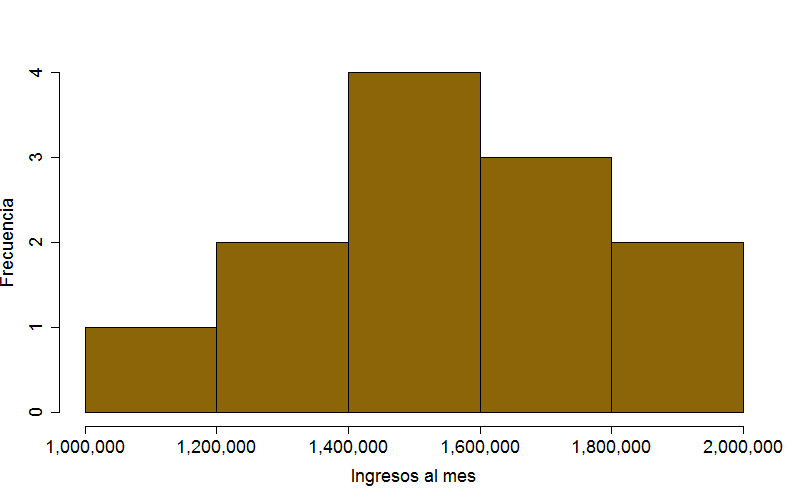
\includegraphics[width=0.4\textwidth]{Avion.png}}%
\hfill
\subcaptionbox{Gráfico con información de la media de ingresos turísticos por la vía Aérea.}{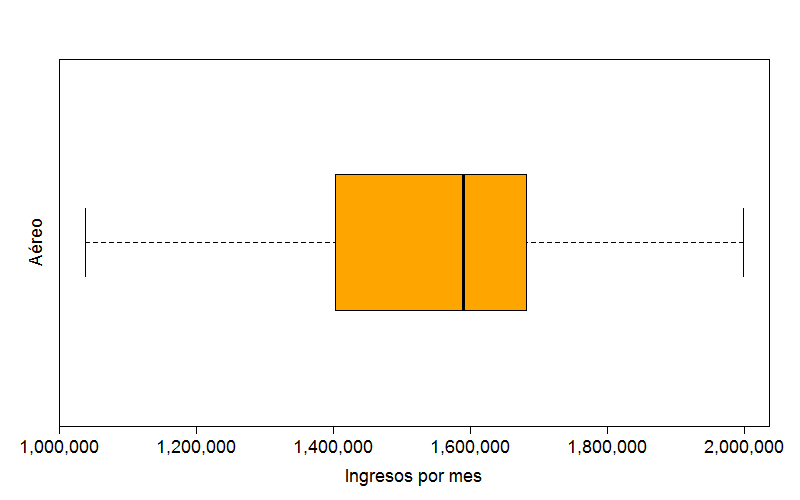
\includegraphics[width=0.4\textwidth]{AvionB.png}}%
\hfill

\caption{Gráficos que muestran el ingreso de turistas al país cada mes por medio de la vía Aérea.}
\label{fig:Avion}
\end{figure}

\begin{figure}[b]
\centering
\subcaptionbox{Histograma que muestra la frecuencia de turistas ingresados al mes por la vía marítima.}{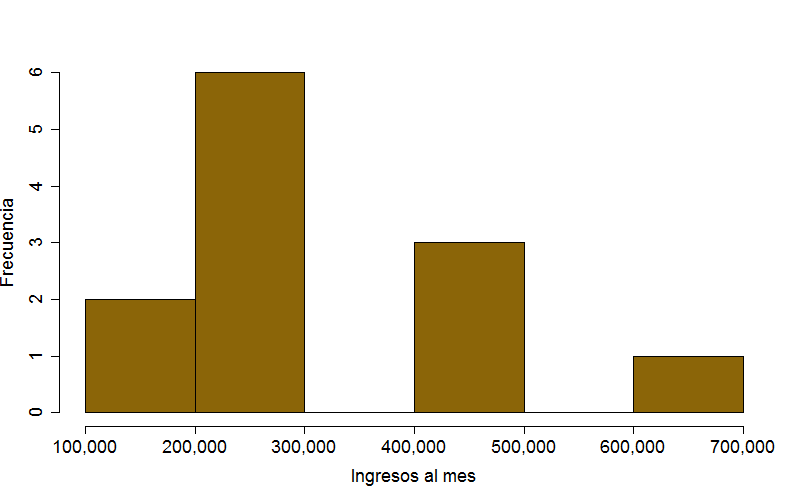
\includegraphics[width=0.4\textwidth]{Maritimo.png}}%
\hfill
\subcaptionbox{Gráfico con información de la media de ingresos turísticos por la vía marítima.}{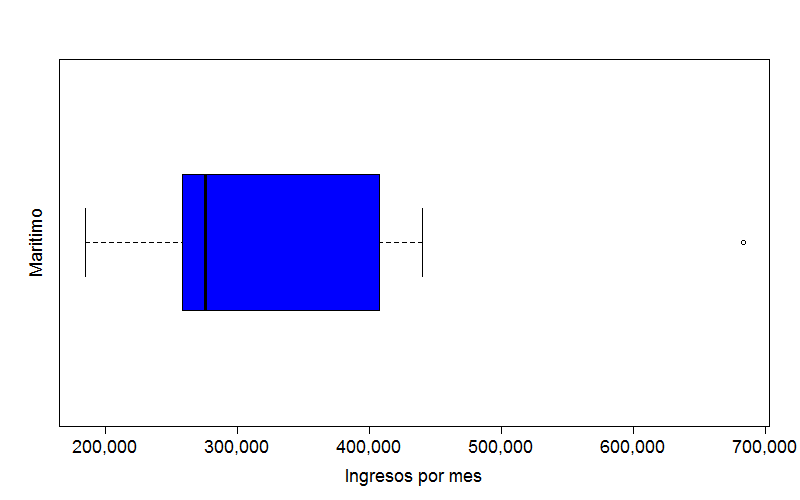
\includegraphics[width=0.4\textwidth]{MaritimoB.png}}%
\hfill

\caption{Gráficos que muestran el ingreso de turistas al país cada mes por medio de la vía marítima.}
\label{fig:Maritimo}
\end{figure}


\begin{figure}[b]
\centering
\subcaptionbox{Histograma que muestra la frecuencia de turistas ingresados al mes por la vía terrestre.}{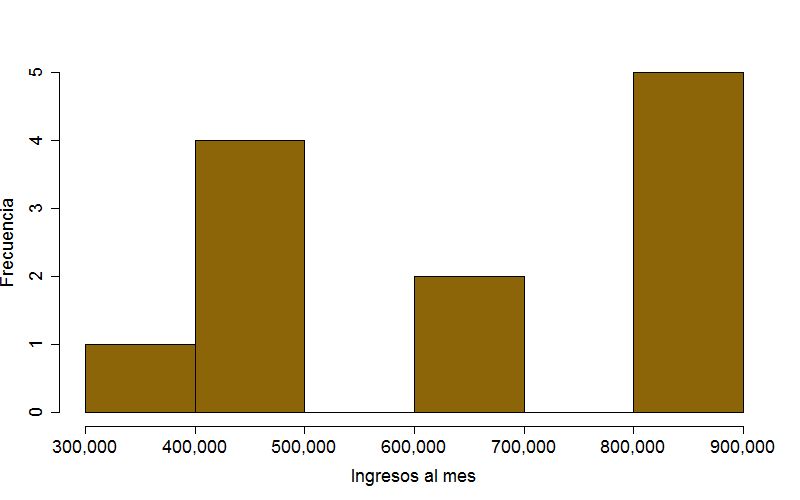
\includegraphics[width=0.4\textwidth]{Terrestre.png}}%
\hfill
\subcaptionbox{Gráfico con información de la media de ingresos turísticos por la vía terrestre.}{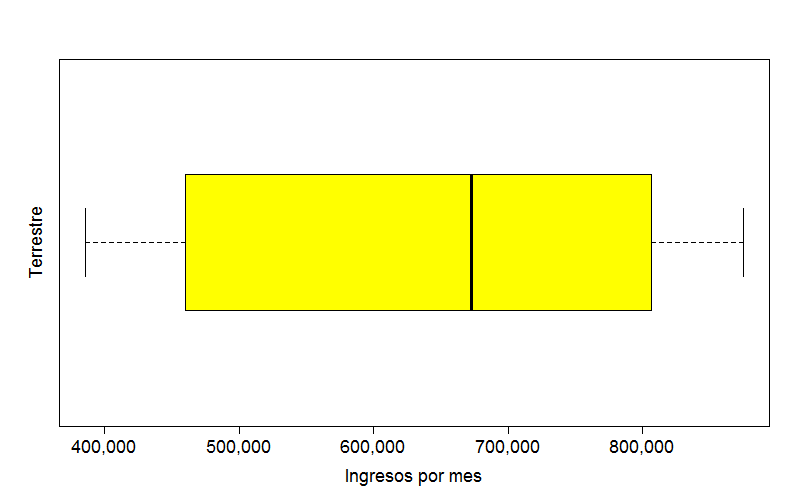
\includegraphics[width=0.4\textwidth]{TerrestreB.png}}%
\hfill

\caption{Gráficos que muestran el ingreso de turistas al país cada mes por medio de la vía terrestre.}
\label{fig:Terrestre}
\end{figure}

 \clearpage 

\printbibliography[title={Referencias}]
\end{document}
